% Los objetivos específicos de cada uno de los subproyectos participantes, enumerándolos brevemente, con claridad, precisión y de manera realista (acorde con la duración prevista del proyecto).
%
% En los subproyectos con dos investigadores principales, deberá indicarse expresamente de qué objetivos específicos se hará responsable cada uno de ellos.
%

\subsubsection*{Objectives of the ENG subproject}

\begin{figure}[h!]
\begin{center}
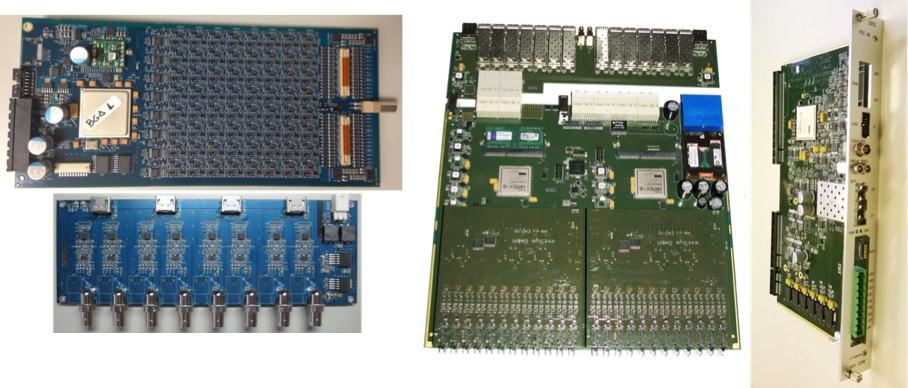
\includegraphics[width=0.9\textwidth]{img/Electronics.jpg}
\end{center}
\caption{\label{Fig:FEE} Left: Front-end boards for SiPM (top) and PMTs (bottom) for NEW and NEXT-100; right: SRS FEC modules in ATCA form factor (left) and “SRS classic” flavour (right) }
\end{figure}

The ENG subproject centralises the front-end electronics, data acquisition (DAQ), online system and slow controls of the NEW and NEXT-100 detectors. It is coordinated by the UPV.
NEXT (via the UPV team) has co-developed a new readout and DAQ concept named SRS \footcite{Toledo2011,SRS2013},for the international RD-51 collaboration at CERN. NEXT front-end modules are connected via copper links to the SRS DAQ interface modules. the CERN standard DATE environment is used as DAQ software. This brings a number of advantages, like counting on a large base of users and developers, reducing production costs and profiting from other group’s developments. SRS has been successfully used in NEXT-DEMO (PMT and SiPM readout, DAQ interface and trigger modules)\footcite{Gil2012,Herrero2012,Esteve2012} and newer versions of these modules are to be used in NEW and NEXT-100\footnote{J.Toledo et al., “The Front-end Electronics for the 1.8-kchannel SiPM Tracking Plane in the NEW Detector,”  presented at TWEPP 2014 (Aix-en-Provence, Sept. 2014)}.

The specific objectives of this sub-project are:

\begin{enumerate}

\item {\bf FEE (Front End Electronics)}: Design, fabrication and commissioning of the front-end electronics for the PMTs and the SiPMs for NEW and NEXT-100. The NP leader is the co-PI of the subproject, Prof. Francisco Toledo (UPV).
\begin{enumerate}
\item	{\em Commissioning NEW front-end electronics in 2015}. As an outcome from two previous projects (CUP and FIS2012-37947-C04-04), the front-end electronics for both the PMT plane and the SiPM plane in NEW are available. The former is already being used in NEXT-DEMO while the latter, an evolution from the NEXT-DEMO electronics, exists as prototype boards and will be available in adequate quantities by the end of 2014. Required cabling, power supplies and mechanical structures have already been purchased.
These electronics will be tested at IFIC in Q1’15 and at the LSC in Q2’15. A study on reliability, performance and signal noise will be carried out during the commissioning phase, resulting either on the final validation of the current designs or on a proposal for changes. In this case, the changes will be carried out in Q4’15 and Q1’16.

\item {\em Production, installation and test of NEXT-100 front-end electronics in 2016}. Lessons learnt with NEW commissioning and initial operation will lead to a document on recommendations for installation and operation of electronics in NEXT-100. The specificity of LSC in terms of grounding and power distribution in the experimental area, together from noise in the power lines and generated by neighbouring experiments, will determine the required noise-reduction techniques (mostly ground connections and ad-hoc filtering). After completing the eventual modifications in the front-end modules (Q1'15), production for NEXT-100 in Q2’16, and Q3'16, module test in Q4’16 will complete the 2016 work plan.

\item {\em Commissioning and Operation of NEXT-100 front-end electronics in 2017}. Potential problems found after installation in a detector of the size of NEXT-100 will be addressed. Front-end firmware may require fine adjustments to (1) ease later energy measurement and tracking algorithms and (2) adjust the trigger algorithms as specified for the different physics campaigns. Commissioning is scheduled for Q1-Q2’17. Operations starts on the second half of the year.
\end{enumerate}
 
\item {\bf DAQ}: Design, fabrication and commissioning of the data acquisition modules for NEW and NEXT-100. The NP leader is the second co-PI of the subproject, Prof. Raul Esteve (UPV).

\begin{enumerate}

\item	{\em Commissioning NEW DAQ interface electronics in 2015}. The DAQ interface modules for NEW and NEXT-100 are also available in two flavours: “classic” SRS modules (19” Eurocard form factor, available from CERN Store) and industry-standard ATCA SRS modules. NEW DAQ will use in a first stage modules from both flavours.

These electronics will be tested at IFIC in Q1’15 and at LSC in Q2’15. A study on reliability and performance will be carried out during the commissioning phase, allowing to choose the best solution for NEW and NEXT-100. 
%A third option, a new SRS solution for very-close-to-detector readout codenamed OC-Box, which is to be developed in collaboration with RD51 and intended as an upgrade for NEXT, will be evaluated in 2015 as a future upgrade. It is based on newer FPGA technology and can replace current FEC modules.

\item	{\em Production, installation and test of NEXT-100 DAQ electronics in 2016}. Lessons learnt with NEW commissioning and initial operation will lead to a decision to go for “classic” or ATCA SRS flavor. Purchases for NEXT-100 in Q2’16, module test and firmware upgrade in Q3’16 and installation in Q4’16 will complete the 2016 work plan.

\item	{\em Commissioning and Operation of NEXT-100 DAQ electronics in 2017}. DAQ performance and functionalities will be verified and adjusted to meet final NEXT-100 requirements. DAQ firmware may require some modifications to (1) ease energy measurement and tracking algorithms and (2) adjust the trigger algorithms as specified.

%\item	NEXT-100 operation in 2018. The DAQ requires no maintenance during operation other than module replacement due to damage or malfunctioning. Placed outside the lead castle in 19” racks next to the front-end modules, the DAQ electronics are easily accessible.

\end{enumerate}

\item {\bf Slow control}: Design, fabrication and commissioning of the slow control for NEW and NEXT-100. The project leader is technical engineer Vicente Álvarez, under the supervision of co-IP J. Toledo. The goals are (1) monitor critical detector parameters, mostly temperature and pressure, (2) control power supplies for the sensors, detector grids and electronics and (3) implement an automatic emergency response monitor.
Six subsystems or partitions have been defined: (1) high-voltage sources for PMTs, (2) low-voltage sources for SiPMs and electronics, (3) high-voltage for grids, (4) gas system status -getters, pump and gas recirculation-, (5) a group of temperature and pressure sensors and (6) the main control panel (with cameras and status overview). Partitions are interconnected via Ethernet. Basic functionalities for all subsystems have been implemented in 2014.

%Power supplies for PMTs and SiPMs are directly controlled to Ethernet. Power supplies for the electronics are controller from a PC via USB, being this PC connected to Ethernet. The other subsystems are controlled via a National Instrument’s Compact-RIO chassis with Ethernet link, embedded in a so-called “Slow Control Box”, which includes relays and connections. A LabView software application will be used for the main control panel.

\begin{enumerate}
\item {\em Design, production and commissioning NEW slow-controls in 2015}. The Slow Controls for NEW will be completed in Q4’14, tested and debugged in  Q1’15 and installed in LSC in Q2’15.

%\item {\em Production, installation and commissioning of NEXT-100 slow-controls electronics}. Monitoring the gas subsystem will be an addition to the Slow Controls for NEXT-100 in 2016.
\end{enumerate}

\item {\bf Online}: Design and commissioning of the online system for NEW and NEXT-100. Interfaces with offline, DAQ and Slow Control. The project leader is Dr. Raúl Esteve. The Online System for NEW comprises the following subsystems: (1) Data Storage, (b) Backup Storage, (c) Pre-processing and (d) Online Monitoring. The DAQ System (a PC farm comprising Local and Global Data Concentrators) produces approx. 30 MByte/s in NEW, which are stored into the NEW Data Storage (up to 8 servers with 8 disks each for up to 65 TByte). The Data Storage has power redundancy and multiple network cards per PC for enhanced reliability. Long-term data selected by the Offline System are stored into the Backup Storage (composed of a server PC and a tape server using 1.5 TByte tapes). The Pre-processing comprises two servers which read event data from the Data Storage and apply a format for later offline processing. Finally, a server in the Online Monitoring is used to gather statics, measure performance, find out bottlenecks and check the health of the different subsystems. A 1-Gb Ethernet switch interconnects the PC servers in the Online System, using virtual LANs to separate different data flows.
Backup Storage, Pre-Processing, Data Storage and Online Monitoring have been tested.
%\begin{enumerate}
%\item {\em Commissioning NEW Online system in 2015}. Required hardware elements have either been already purchased of will be purchased before the end of 2014. Prototypes for each sub-system have been already constructed and tested in 2014. The main task in 2015 is to tune the system for NEW operation.
%\item {\em Production, installation and test of NEXT-100 in 2016}. The Online System architecture for NEW is valid for NEXT-100. The main difference is a higher throughput, requiring the use of 10 Gb Ethernet instead of 1Gb Ethernet and the addition of a few servers as a result of the higher data load.
%\end{enumerate}

\end{enumerate}

%\subsubsection*{Expected difficulties and contingency plan}
%
%Potential difficulties that could arise as a result of NEW operation in Canfranc are: power line noise, grounding scheme, noise from neighbouring experiments and potential power consumption limitations during power-up. A power-up sequence must be defined to limit the peak AC current, which can be high in an experiment of the size of NEXT-100.
%
%Usual precautions have been taken in the front-end to deal with noisy environments (differential input stages and shielded cables), as well as other counter-measures are foreseen for the AC power line inputs (low-pass filters and transient suppressors) and low-voltage DC lines (common mode filters, overvoltage and overcurrent protections). 
%
%Previous experience with NEXT-DEMO and the current developments for NEW provides us enough confidence on the operation of the front-end, DAQ and online system. Still, each experimental area poses its own electrical and grounding challenges and LSC may not be an exception.
%
%A contingency plan may include additional budget to address unexpected noise sources and electrical problems which may only show up in a large installation. Measures may include enhanced cable shields or simply more expensive cabling, additional filtering and transient suppressors and enhanced grounding scheme. The additional cost is difficult to estimate and therefore is included as a part of the overall experiment contingency budget.
%
%

%
%\subsubsection*{ENG subproject: schedule}
%
%
%\begin{figure}[h!]
%\begin{center}
%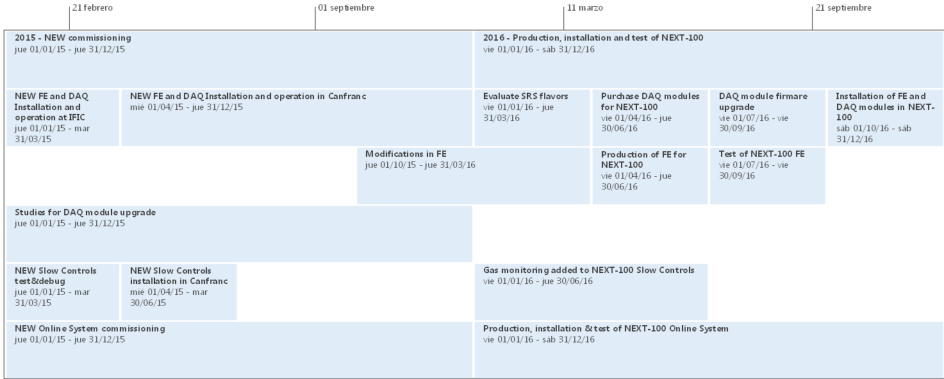
\includegraphics[width=0.99\textwidth]{img/ENF_CRONO.pdf}
%\end{center}
%\caption{\label{Fig:CronoEng} Cronogram for the ENG subproject. }
%\end{figure}
%
%\subsubsection*{Justification for the requested personnel}
%
%Two positions are requested with the following profiles:
%\begin{enumerate}
%\item	Electronics technician or BSc in Electronics Engineering, requested for three years of the Project (30 k\euro/year). Will carry out installation, maintenance, repairing and support of the front-end and DAQ interface electronics for NEW and NEXT-100, as well as the power supplies for sensors and electronics. Will also take part in the design and construction of small circuits (like filters or cabling). Will help in the commissioning phases and in the coordination of the electronic modules purchases and production and will carry out functional tests of the new units. Based in Valencia, will travel to LSC for installation and maintenance.
%
%\item Computer scientist/engineer (BSc or MSc), requested for four years (40 k\euro/year). Must be expert in Linux systems administration and Ethernet computer networks. Will configure, administer, maintain and support the different PC clusters (mostly running CERN Scientific Linux) in the DAQ, Online and Offline systems. Will configure the DATE environment for the DAQ system. Will scale these systems according to specific needs (like the upgrade from NEW to NEXT-100). Will manage the data storage. Will carry out R\&D programs to enhance performance. Construction and commissioning. Based in Valencia, will travel to Canfranc for installation and maintenance.
%
%\end{enumerate}
%
